\documentclass[polish,envcountsect,10pt]{beamer}
\usetheme{metropolis}
\usepackage[T1]{fontenc}
\usepackage{polski}
\usepackage{babel}
\usepackage{tikz}
\usepackage{xcolor}

\title{Triangulacja i diagramy Voronoi}
\author{Krzysztof Nasuta}
\date{Gdańsk, 2025}

\begin{document}

\frame{\titlepage}

\begin{frame}{Ogólna definicja triangulacji}
  \frametitle{Ogólna definicja triangulacji}
  Triangulacja to proces \textbf{podziału płaszczyzny bądź wielokąta na zbiór trójkątów}, zazwyczaj w taki sposób, aby bok trójkąta należał w całości do dokładnie dwóch trójkątów obok siebie.

  \begin{center}
    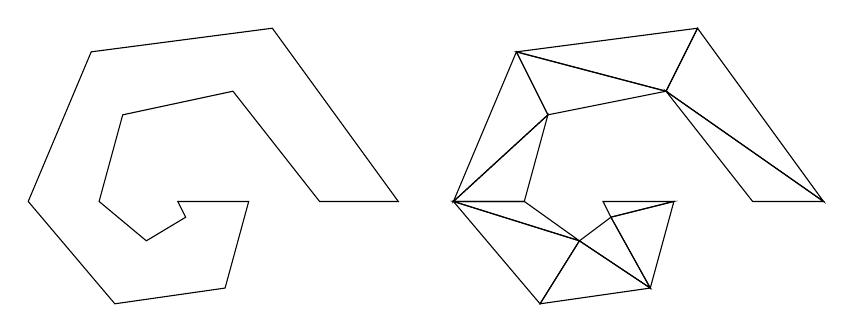
\begin{tikzpicture}
      \draw (1.3, 1.5) -- (1.6, 2.6) -- (3.0, 2.9) -- (4.1, 1.5) -- (5.1, 1.5) -- (3.5, 3.7) -- (1.2, 3.4) -- (0.4, 1.5) -- (1.5, 0.2) -- (2.9, 0.4) -- (3.2, 1.5) -- (2.3, 1.5) -- (2.4, 1.3) -- (1.9, 1.0) -- cycle;

      \pause
      \draw (7.8, 1.3) -- (7.4, 1.0) -- (8.3, 0.4) -- cycle;
      \draw (7.8, 1.3) -- (8.3, 0.4) -- (8.6, 1.5) -- cycle;
      \draw (7.8, 1.3) -- (8.6, 1.5) -- (7.7, 1.5) -- cycle;
      \draw (6.9, 0.2) -- (8.3, 0.4) -- (7.4, 1.0) -- cycle;
      \draw (6.9, 0.2) -- (7.4, 1.0) -- (5.8, 1.5) -- cycle;
      \draw (5.8, 1.5) -- (7.4, 1.0) -- (6.7, 1.5) -- cycle;
      \draw (5.8, 1.5) -- (6.7, 1.5) -- (7.0, 2.6) -- cycle;
      \draw (5.8, 1.5) -- (7.0, 2.6) -- (6.6, 3.4) -- cycle;
      \draw (7.0, 2.6) -- (8.5, 2.9) -- (6.6, 3.4) -- cycle;
      \draw (9.6, 1.5) -- (10.5, 1.5) -- (8.5, 2.9) -- cycle;
      \draw (8.9, 3.7) -- (6.6, 3.4) -- (8.5, 2.9) -- cycle;
      \draw (8.9, 3.7) -- (8.5, 2.9) -- (10.5, 1.5) -- cycle;
    \end{tikzpicture}
  \end{center}
\end{frame}

\begin{frame}{Definicje triangulacji w różnych dziedzinach matematyki}
  \frametitle{Definicje triangulacji w różnych dziedzinach matematyki}
  \begin{itemize}
    \item W geometrii triangulacja odnosi się do podziału płaszczyzny euklidesowej na trójkąty. W ogólności mówimy o \textbf{podziale przestrzeni euklidesowej na simpleksy}.
      \pause
    \item W teorii grafów występują dwie definicje triangulacji:
      \begin{itemize}
        \item \textbf{Tworzenie grafów maksymalnie planarnych}, czyli takich, do których nie można dodać żadnej krawędzi bez utraty własności planarnych. W grafie takim każda ścina jest trójkątem.
          \pause
        \item \textbf{Dodawanie krawędzi do grafu w celu otrzymania grafu cięciwowego}, czyli takiego, w którym każdy cykl o długości czterech lub większej ma przekątną.
      \end{itemize}
  \end{itemize}
\end{frame}

\begin{frame}{Źródła}
  \frametitle{Źródła}
  \begin{thebibliography}{1}
    \bibitem{1} \url{https://mathworld.wolfram.com/Triangulation.html}
    \bibitem{2} \url{https://en.wikipedia.org/wiki/Triangulation_(disambiguation)}
  \end{thebibliography}
\end{frame}

\end{document}
